\chapter{Further Plots and Tables}
\label{ap:more_plots}

\section{t-SNE plots for the data from \cite{Derrac2015}}

\begin{figure}[h]
	\begin{center}
	  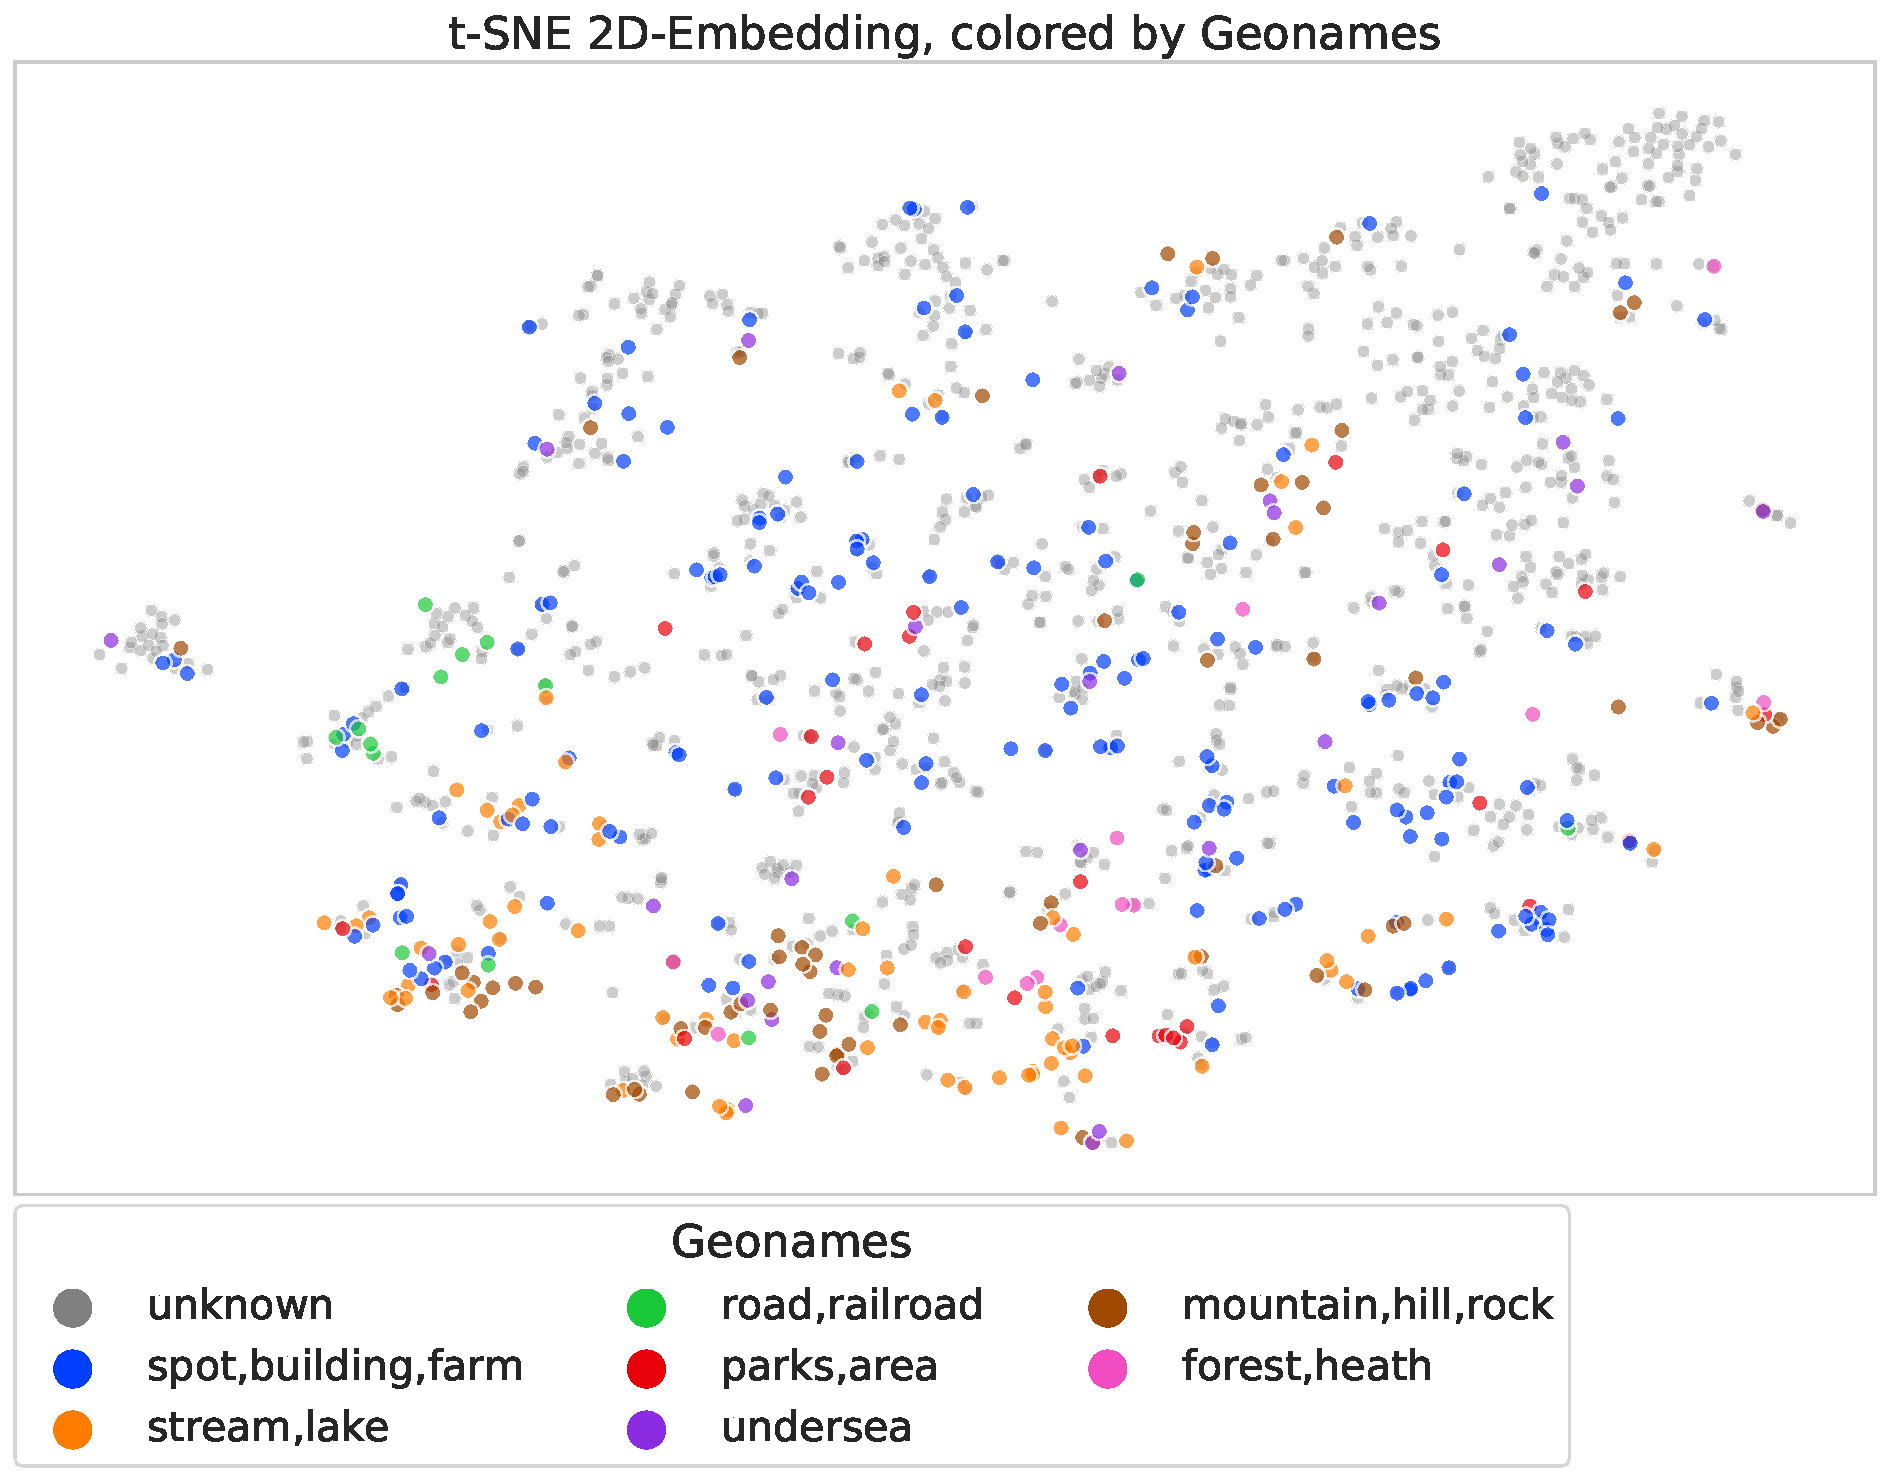
\includegraphics[width=\textwidth]{graphics/figures/scatter_mds_tsne_places_Geonames.pdf}
	  \slcaption{2D Visualization of the Placetypes-Dissimilarity-Matrix \todoparagraph{not mine, but the one of Derrac}, generated with \gls{tsne}. See \url{https://github.com/cstenkamp/derive_conceptualspaces/blob/main/notebooks/text_referenced_plots/desc15_mds_2d3d.ipynb} for the origin of this plot.}
	  \label{fig:scatter_mds_placetypes}
      %TODO: "colored by Geonames"
	\end{center}
\end{figure}


\begin{figure}[h]
	\begin{center}
	  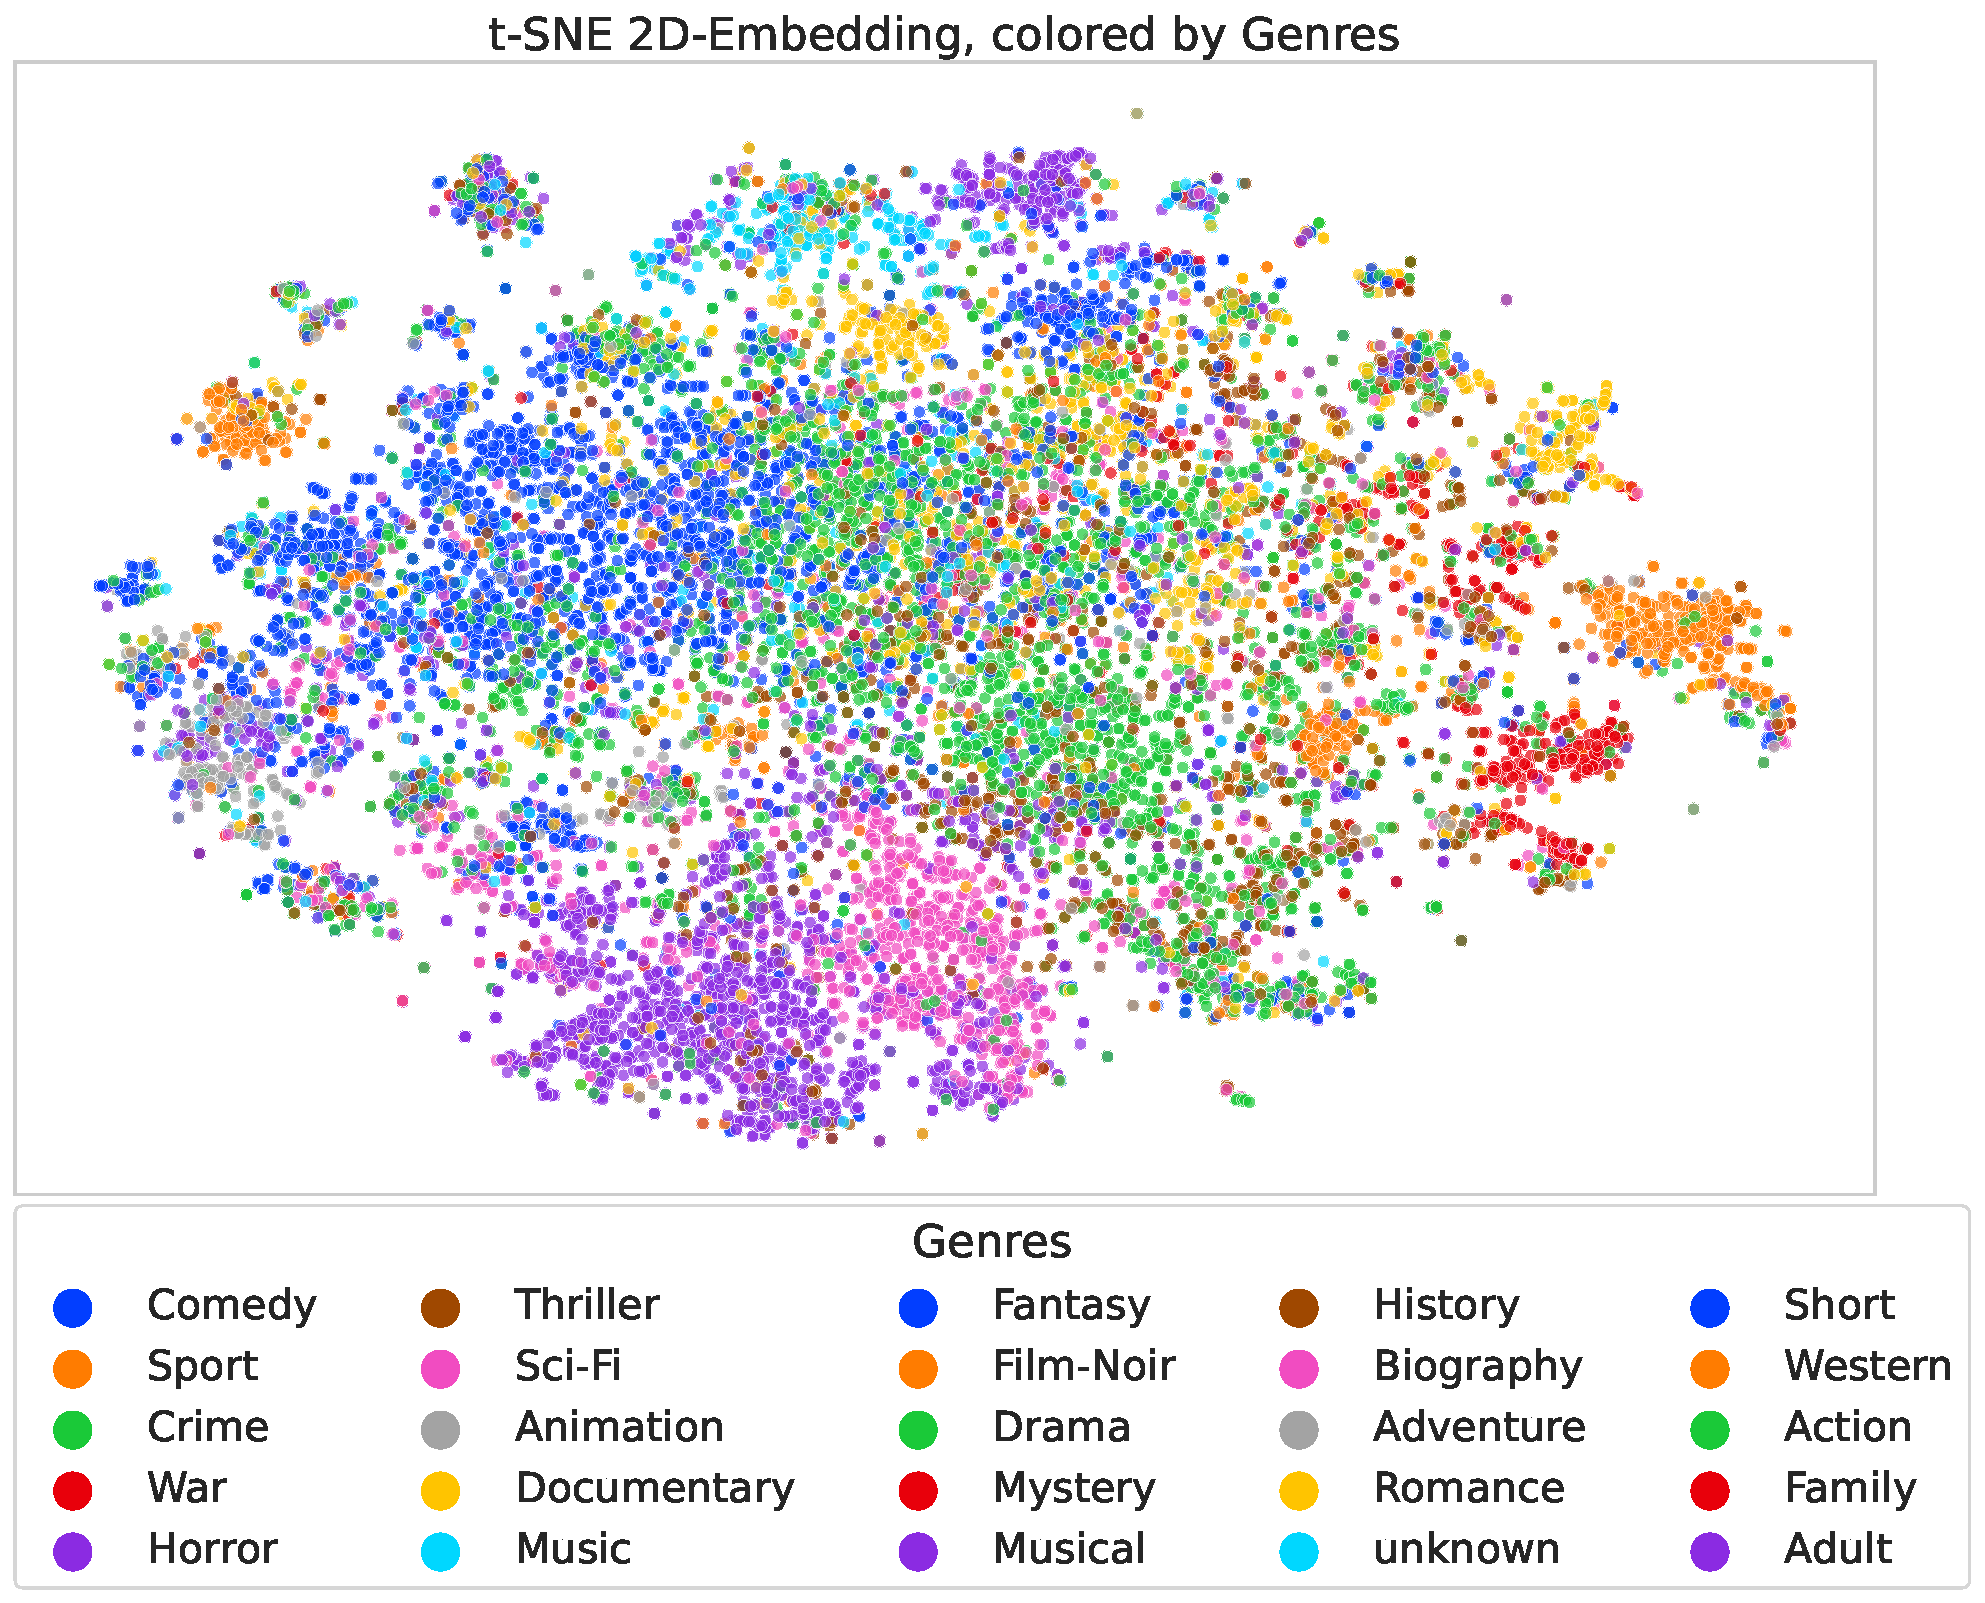
\includegraphics[width=\textwidth]{graphics/figures/scatter_mds_tsne_movies_Genres.pdf}
	  \slcaption{2D Visualization of the Movie-Dissimilarity-Matrix, generated with \gls{tsne}. See \url{https://github.com/cstenkamp/derive_conceptualspaces/blob/main/notebooks/text_referenced_plots/desc15_mds_2d3d.ipynb} for the origin of this plot.}
	  \label{fig:scatter_mds_movies}
      %TODO: "colored by genre"
	\end{center}
\end{figure}


\todoparagraph{Note that at} \url{https://github.com/cstenkamp/derive_conceptualspaces/blob/main/notebooks/text_referenced_plots/desc15_mds_2d3d.ipynb} there are also interactive 3D-Versions of these plots. The one for the SIDDATA-dataset is at \url{https://github.com/cstenkamp/derive_conceptualspaces/blob/main/notebooks/text_referenced_plots/visualize_embeddings.ipynb}, also 2D and interactive 3D. 

\clearpage
\section{Results for Classifiers on placetypes}

\begin{table}[H]
	\centering
	\makebox[\textwidth][c]{
		\resizebox{1.2\textwidth}{!}{%
		\begin{tabular}{rr|ccccc|ccccc|cc|cc}
		&
		&
		\multicolumn{5}{c|}{\textbf{\textcite{Alshaikh2020} (MDS)}} &
		\multicolumn{5}{c|}{\textbf{\textcite{Ager2018}}} &
		\multicolumn{2}{c|}{\textbf{\textcite{Derrac2015}}} &
		\multicolumn{2}{c}{\textbf{This work}} \\
		&
		&
		\textbf{Random} &
		\textbf{AHC} &
		\textbf{Primary} &
		\textbf{Sub} &
		\textbf{Ortho} &
		\textbf{FT MDS} &
		\textbf{MDS} &
		\textbf{FT AWV} &
		\textbf{AWV} &
		\textbf{LDA} &
		\textbf{Best} &
		\textbf{Best BL} &
		\textbf{Best-all} &
		\textbf{Mean-Best} \\ \midrule
		\textbf{Foursquare} &
		\textbf{D1} &
		0.39 &
		0.36 &
		0.36 &
		0.43 &
		\textbf{0.45} &
		0.41 &
		0.38 &
		0.39 &
		0.32 &
		\textbf{0.55} &
		\multicolumn{2}{c|}{-} &
		\textbf{0.50} & 0.45
		\\
		&
		\textbf{D3} &
		0.50 &
		0.46 &
		0.48 &
		0.54 &
		\textbf{0.57} &
		0.44 &
		0.42 &
		0.42 &
		0.37 &
		0.48 &
		\multicolumn{2}{c|}{-} &
		\textbf{0.58} & 0.5
		\\
		&
		\textbf{DN} &
		\multicolumn{5}{c|}{-} &
		0.41 &
		0.42 &
		0.41 &
		0.31 &
		0.47 &
		\textbf{0.53} &
		\textbf{0.53} &
		\textbf{0.57} & 0.55
		\\
		\multicolumn{1}{l}{} &
		\multicolumn{1}{l|}{\textbf{Any}} &
		\multicolumn{5}{c|}{-} &
		\multicolumn{5}{c|}{-} &
		\textbf{0.73} &
		0.72 &
		- & -
		\\
		\textbf{Geonames} &
		\textbf{D1} &
		0.23 &
		0.22 &
		0.24 &
		0.20 &
		0.28 &
		0.32 &
		\textbf{0.32} &
		0.31 &
		0.28 &
		\textbf{0.34} &
		\multicolumn{2}{c|}{-} &
		\textbf{0.51} & 0.48
		\\
		&
		\textbf{D3} &
		0.27 &
		0.29 &
		0.27 &
		0.32 &
		\textbf{0.34} &
		0.31 &
		0.31 &
		0.29 &
		0.28 &
		0.32 &
		\multicolumn{2}{c|}{-} &
		\textbf{0.54} & 0.51
		\\
		&
		\textbf{DN} &
		\multicolumn{5}{c|}{-} &
		0.24 &
		0.21 &
		0.23 &
		0.22 &
		0.27 &
		\textbf{0.37} &
		0.2 &
		\textbf{0.46} & 0.44
		\\
		\multicolumn{1}{l}{} &
		\multicolumn{1}{l|}{\textbf{Any}} &
		\multicolumn{5}{c|}{-} &
		\multicolumn{5}{c|}{-} &
		\textbf{0.41} &
		0.36 &
		- & -
		
		\end{tabular}%
		} % resizebox
	} % makebox
	\caption{F1-Scores of classifiers predicting GeoNames- and Foursquare-labels for baselines, \mainalgos and this work (long)}
	\label{tab:f1_placetypes_long}
\end{table}


\autoref{tab:f1_placetypes_long} is a longer version of \autoref{tab:f1_mainalgos_me_short}, reporting F1-Scores of classifiers predicting GeoNames- and Foursquare-labels for baselines, \mainalgos and this work. 
\textbf{Cls} column encodes the classifier: \textbf{D1/3} are \glspl{dt} of depth 1/3, \textbf{DN} an unbounded \gls{dt}. Condition \textbf{Any} refers to the best of all semantic classifiers developed by \cite{Derrac2015}. \\
First five columns are the exact results reported by \cite{Alshaikh2020}, next five columns those by \cite{Ager2018}, afterwards the best config of \cite{Derrac2015} and the best baseline-condition of \cite{Derrac2015}. The exact conditions of that work are (left to right, top to bottom): C4.5\textsubscript{dir}, C4.5\textsubscript{MDS}, Col, 1-NN (100D), C4.5\textsubscript{dir}, C4.5\textsubscript{MDS}, Analog\textsubscript{C}, 1-NN (50D). Explanations of the respective conditions can be found in their work. \\
All scores are reported with a train-test split of 70\% to 30\%. Note that the reported results of \cite{Ager2018} are unrepresentive when compared to the other datasets: For the placetypes-dataset, \textbf{LDA} performs consistently better than their methods, which is not the case for all other datasets used by them. In the case of \cite{Alshaikh2020}, the results for the placetypes-dataset seem to indicate that the \textbf{Ortho}-condition performs consistently better than the \textbf{Sub}-condition, which was however not the case for any of the other datasets the authors considered. \\
Final columns are the results of this work. Column \textbf{Best-all} encodes a different for each row, specifically the one that yields the best result for the respective classification task, whereas column \textbf{Mean-Best} refers to the single configuration that achieved the best results on average.